\documentclass{standalone}
\usepackage{tikz}
\usetikzlibrary{patterns, positioning}


\begin{document}
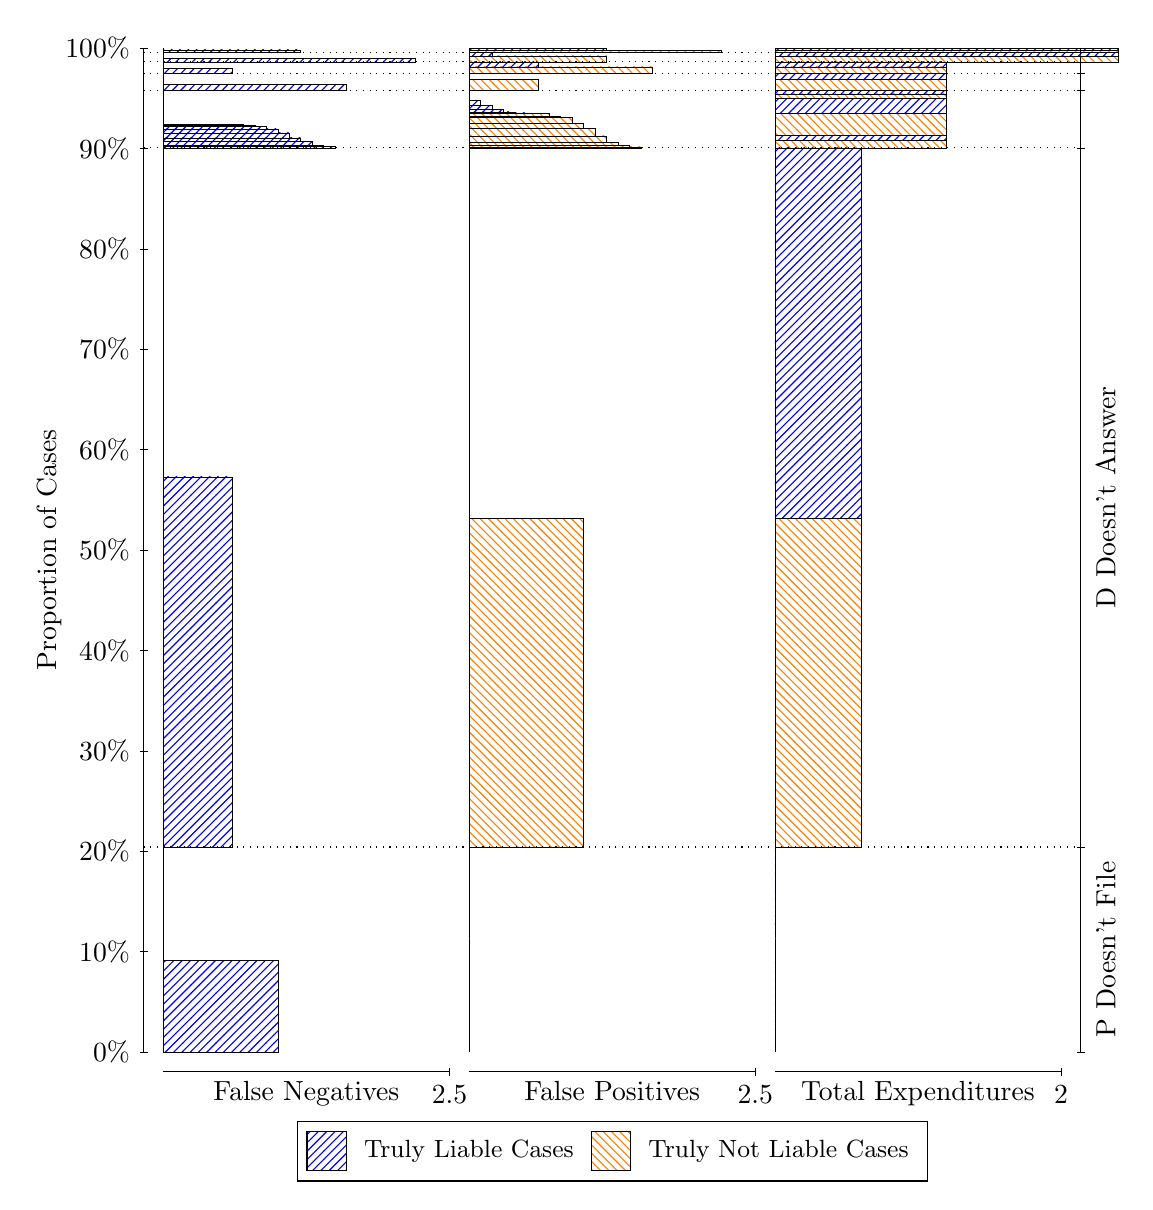
\begin{tikzpicture}
\draw[black, very thin] (1.5,1.75) -- (1.5,14.5);
\node[rotate=90, text=black, anchor=center] at (0.3, 8.125) {Proportion of Cases};
\draw[black, very thin] (1.45,1.75) -- (1.55,1.75);
\node[text=black, anchor=east] at (1.45, 1.75) {0\%};
\draw[black, very thin] (1.45,3.025) -- (1.55,3.025);
\node[text=black, anchor=east] at (1.45, 3.025) {10\%};
\draw[black, very thin] (1.45,4.3) -- (1.55,4.3);
\node[text=black, anchor=east] at (1.45, 4.3) {20\%};
\draw[black, very thin] (1.45,5.575) -- (1.55,5.575);
\node[text=black, anchor=east] at (1.45, 5.575) {30\%};
\draw[black, very thin] (1.45,6.85) -- (1.55,6.85);
\node[text=black, anchor=east] at (1.45, 6.85) {40\%};
\draw[black, very thin] (1.45,8.125) -- (1.55,8.125);
\node[text=black, anchor=east] at (1.45, 8.125) {50\%};
\draw[black, very thin] (1.45,9.4) -- (1.55,9.4);
\node[text=black, anchor=east] at (1.45, 9.4) {60\%};
\draw[black, very thin] (1.45,10.675) -- (1.55,10.675);
\node[text=black, anchor=east] at (1.45, 10.675) {70\%};
\draw[black, very thin] (1.45,11.95) -- (1.55,11.95);
\node[text=black, anchor=east] at (1.45, 11.95) {80\%};
\draw[black, very thin] (1.45,13.225) -- (1.55,13.225);
\node[text=black, anchor=east] at (1.45, 13.225) {90\%};
\draw[black, very thin] (1.45,14.5) -- (1.55,14.5);
\node[text=black, anchor=east] at (1.45, 14.5) {100\%};

\draw[black, very thin] (13.4,1.75) -- (13.4,14.5);
\draw[black, very thin] (13.35,1.75) -- (13.45,1.75);
\node[anchor=west] at (13.35, 1.75) {};
\draw[black, very thin] (13.35,4.3535) -- (13.45,4.3535);
\node[anchor=west] at (13.35, 4.3535) {};
\draw[black, very thin] (13.35,13.232) -- (13.45,13.232);
\node[anchor=west] at (13.35, 13.232) {};
\draw[black, very thin] (13.35,13.964) -- (13.45,13.964);
\node[anchor=west] at (13.35, 13.964) {};
\draw[black, very thin] (13.35,14.176) -- (13.45,14.176);
\node[anchor=west] at (13.35, 14.176) {};
\draw[black, very thin] (13.35,14.325) -- (13.45,14.325);
\node[anchor=west] at (13.35, 14.325) {};
\draw[black, very thin] (13.35,14.448) -- (13.45,14.448);
\node[anchor=west] at (13.35, 14.448) {};
\draw[black, very thin] (13.35,14.5) -- (13.45,14.5);
\node[anchor=west] at (13.35, 14.5) {};

\draw[black, very thin, pattern color=blue, pattern=north east lines] (1.75,1.75) rectangle (3.2033,2.9115);
\draw[black, very thin, pattern color=orange, pattern=north west lines] (1.75,2.9115) rectangle (1.75,4.3535);
\draw[black, very thin, pattern color=blue, pattern=north east lines] (1.75,4.3535) rectangle (2.622,9.0548);
\draw[black, very thin, pattern color=orange, pattern=north west lines] (1.75,9.0548) rectangle (1.75,13.232);
\draw[black, very thin, pattern color=blue, pattern=north east lines] (1.75,13.232) rectangle (3.93,13.254);
\draw[black, very thin, pattern color=blue, pattern=north east lines] (1.75,13.254) rectangle (3.7847,13.268);
\draw[black, very thin, pattern color=blue, pattern=north east lines] (1.75,13.268) rectangle (3.6393,13.317);
\draw[black, very thin, pattern color=blue, pattern=north east lines] (1.75,13.317) rectangle (3.494,13.358);
\draw[black, very thin, pattern color=blue, pattern=north east lines] (1.75,13.358) rectangle (3.3487,13.421);
\draw[black, very thin, pattern color=blue, pattern=north east lines] (1.75,13.421) rectangle (3.2033,13.473);
\draw[black, very thin, pattern color=blue, pattern=north east lines] (1.75,13.473) rectangle (3.058,13.507);
\draw[black, very thin, pattern color=blue, pattern=north east lines] (1.75,13.507) rectangle (2.9127,13.52);
\draw[black, very thin, pattern color=blue, pattern=north east lines] (1.75,13.52) rectangle (2.7673,13.528);
\draw[black, very thin, pattern color=orange, pattern=north west lines] (1.75,13.528) rectangle (1.75,13.964);
\draw[black, very thin, pattern color=blue, pattern=north east lines] (1.75,13.964) rectangle (4.0753,14.042);
\draw[black, very thin, pattern color=orange, pattern=north west lines] (1.75,14.042) rectangle (1.75,14.176);
\draw[black, very thin, pattern color=blue, pattern=north east lines] (1.75,14.176) rectangle (2.622,14.241);
\draw[black, very thin, pattern color=orange, pattern=north west lines] (1.75,14.241) rectangle (1.75,14.325);
\draw[black, very thin, pattern color=blue, pattern=north east lines] (1.75,14.325) rectangle (4.9473,14.372);
\draw[black, very thin, pattern color=orange, pattern=north west lines] (1.75,14.372) rectangle (1.75,14.448);
\draw[black, very thin, pattern color=blue, pattern=north east lines] (1.75,14.448) rectangle (3.494,14.475);
\draw[black, very thin, pattern color=orange, pattern=north west lines] (1.75,14.475) rectangle (1.75,14.5);
\draw[black, very thin, pattern color=orange, pattern=north west lines] (5.6333,1.75) rectangle (5.6333,3.192);
\draw[black, very thin, pattern color=blue, pattern=north east lines] (5.6333,3.192) rectangle (5.6333,4.3535);
\draw[black, very thin, pattern color=orange, pattern=north west lines] (5.6333,4.3535) rectangle (7.0867,8.531);
\draw[black, very thin, pattern color=blue, pattern=north east lines] (5.6333,8.531) rectangle (5.6333,13.232);
\draw[black, very thin, pattern color=orange, pattern=north west lines] (5.6333,13.232) rectangle (7.8133,13.244);
\draw[black, very thin, pattern color=orange, pattern=north west lines] (5.6333,13.244) rectangle (7.668,13.26);
\draw[black, very thin, pattern color=orange, pattern=north west lines] (5.6333,13.26) rectangle (7.5227,13.306);
\draw[black, very thin, pattern color=orange, pattern=north west lines] (5.6333,13.306) rectangle (7.3773,13.383);
\draw[black, very thin, pattern color=orange, pattern=north west lines] (5.6333,13.383) rectangle (7.232,13.478);
\draw[black, very thin, pattern color=orange, pattern=north west lines] (5.6333,13.478) rectangle (7.0867,13.542);
\draw[black, very thin, pattern color=orange, pattern=north west lines] (5.6333,13.542) rectangle (6.9413,13.616);
\draw[black, very thin, pattern color=orange, pattern=north west lines] (5.6333,13.616) rectangle (6.796,13.636);
\draw[black, very thin, pattern color=orange, pattern=north west lines] (5.6333,13.636) rectangle (6.6507,13.669);
\draw[black, very thin, pattern color=blue, pattern=north east lines] (5.6333,13.669) rectangle (6.36,13.677);
\draw[black, very thin, pattern color=blue, pattern=north east lines] (5.6333,13.677) rectangle (6.2147,13.689);
\draw[black, very thin, pattern color=blue, pattern=north east lines] (5.6333,13.689) rectangle (6.0693,13.724);
\draw[black, very thin, pattern color=blue, pattern=north east lines] (5.6333,13.724) rectangle (5.924,13.775);
\draw[black, very thin, pattern color=blue, pattern=north east lines] (5.6333,13.775) rectangle (5.7787,13.838);
\draw[black, very thin, pattern color=blue, pattern=north east lines] (5.6333,13.838) rectangle (5.6333,13.964);
\draw[black, very thin, pattern color=orange, pattern=north west lines] (5.6333,13.964) rectangle (6.5053,14.099);
\draw[black, very thin, pattern color=blue, pattern=north east lines] (5.6333,14.099) rectangle (5.6333,14.176);
\draw[black, very thin, pattern color=orange, pattern=north west lines] (5.6333,14.176) rectangle (7.9587,14.26);
\draw[black, very thin, pattern color=blue, pattern=north east lines] (5.6333,14.26) rectangle (6.5053,14.325);
\draw[black, very thin, pattern color=orange, pattern=north west lines] (5.6333,14.325) rectangle (7.3773,14.401);
\draw[black, very thin, pattern color=blue, pattern=north east lines] (5.6333,14.401) rectangle (5.924,14.448);
\draw[black, very thin, pattern color=orange, pattern=north west lines] (5.6333,14.448) rectangle (8.8307,14.472);
\draw[black, very thin, pattern color=blue, pattern=north east lines] (5.6333,14.472) rectangle (7.3773,14.5);
\draw[black, very thin, pattern color=orange, pattern=north west lines] (9.5167,1.75) rectangle (9.5167,3.192);
\draw[black, very thin, pattern color=blue, pattern=north east lines] (9.5167,3.192) rectangle (9.5167,4.3535);
\draw[black, very thin, pattern color=orange, pattern=north west lines] (9.5167,4.3535) rectangle (10.607,8.531);
\draw[black, very thin, pattern color=blue, pattern=north east lines] (9.5167,8.531) rectangle (10.607,13.232);
\draw[black, very thin, pattern color=orange, pattern=north west lines] (9.5167,13.232) rectangle (11.697,13.327);
\draw[black, very thin, pattern color=blue, pattern=north east lines] (9.5167,13.327) rectangle (11.697,13.39);
\draw[black, very thin, pattern color=orange, pattern=north west lines] (9.5167,13.39) rectangle (11.697,13.671);
\draw[black, very thin, pattern color=blue, pattern=north east lines] (9.5167,13.671) rectangle (11.697,13.856);
\draw[black, very thin, pattern color=orange, pattern=north west lines] (9.5167,13.856) rectangle (11.697,13.917);
\draw[black, very thin, pattern color=blue, pattern=north east lines] (9.5167,13.917) rectangle (11.697,13.964);
\draw[black, very thin, pattern color=orange, pattern=north west lines] (9.5167,13.964) rectangle (11.697,14.099);
\draw[black, very thin, pattern color=blue, pattern=north east lines] (9.5167,14.099) rectangle (11.697,14.176);
\draw[black, very thin, pattern color=orange, pattern=north west lines] (9.5167,14.176) rectangle (11.697,14.26);
\draw[black, very thin, pattern color=blue, pattern=north east lines] (9.5167,14.26) rectangle (11.697,14.325);
\draw[black, very thin, pattern color=orange, pattern=north west lines] (9.5167,14.325) rectangle (13.877,14.401);
\draw[black, very thin, pattern color=blue, pattern=north east lines] (9.5167,14.401) rectangle (13.877,14.448);
\draw[black, very thin, pattern color=orange, pattern=north west lines] (9.5167,14.448) rectangle (13.877,14.472);
\draw[black, very thin, pattern color=blue, pattern=north east lines] (9.5167,14.472) rectangle (13.877,14.5);
\draw[black, dotted] (1.5,4.3535) -- (13.4,4.3535);
\draw[black, dotted] (1.5,13.232) -- (13.4,13.232);
\draw[black, dotted] (1.5,13.964) -- (13.4,13.964);
\draw[black, dotted] (1.5,14.176) -- (13.4,14.176);
\draw[black, dotted] (1.5,14.325) -- (13.4,14.325);
\draw[black, dotted] (1.5,14.448) -- (13.4,14.448);
\draw[black, very thin] (1.75,1.5) -- (5.3833,1.5);
\node[text=black, anchor=north] at (3.5667, 1.5) {False Negatives};
\draw[black, very thin] (5.3833,1.45) -- (5.3833,1.55);
\node[text=black, anchor=north] at (5.3833, 1.45) {2.5};

\draw[black, very thin] (5.6333,1.5) -- (9.2667,1.5);
\node[text=black, anchor=north] at (7.45, 1.5) {False Positives};
\draw[black, very thin] (9.2667,1.45) -- (9.2667,1.55);
\node[text=black, anchor=north] at (9.2667, 1.45) {2.5};

\draw[black, very thin] (9.5167,1.5) -- (13.15,1.5);
\node[text=black, anchor=north] at (11.333, 1.5) {Total Expenditures};
\draw[black, very thin] (13.15,1.45) -- (13.15,1.55);
\node[text=black, anchor=north] at (13.15, 1.45) {2};

\node[text=black, centered, rotate=90] at (13.72, 3.0517) {P Doesn't File};
\node[text=black, centered, rotate=90] at (13.72, 8.7929) {D Doesn't Answer};






\draw (7.449999999999999,1.5) node[draw=none] (baseCoordinate) {};
\begin{scope}[align=center]
        \matrix[scale=0.5, draw=black, below=0.5cm of baseCoordinate, nodes={draw}, column sep=0.1cm]{
            \node[rectangle, draw, minimum width=0.5cm, minimum height=0.5cm, pattern color=blue, pattern=north east lines] {}; &
            \node[draw=none, font=\small, text=black] (B) {Truly Liable Cases}; &
            \node[rectangle, draw, minimum width=0.5cm, minimum height=0.5cm, pattern color=orange, pattern=north west lines] {}; &
            \node[draw=none, font=\small, text=black] (B) {Truly Not Liable Cases}; \\
            };
\end{scope}

\end{tikzpicture}
\end{document}